% -*- mode: latex; fill-column: 150; -*-
\RequirePackage{fix-cm}
%
\documentclass{article}
\usepackage[pdftex]{graphicx}
\usepackage{epstopdf}
\usepackage{url}
\usepackage{verbatim}
\usepackage{hyphenat}
\usepackage{amsthm}
\renewcommand{\labelitemi}{$\bullet$}
\begin{document}

\title{Algebra Systems}
\author{Debasish Ghosh}

\section{Algebra}
\label{algebra}

Let $ F: C \rightarrow C $ be an endofunctor on category C. An F-algebra is a pair $ (A, \varphi) $ , where A is an object and $ \varphi : FA \rightarrow A $ is an arrow in the category C. The object A is the \textit{carrier} and the functor F is the \textit{signature} of the algebra.

\section{Algebra Homomorphism}
\label{algebrahomomorphism}

Let $(C, \varphi)$ and $(D, \psi)$ be two F-algebras. An F-homomorphism from $(C, \varphi)$ to $(D, \psi)$ is an arrow $f : C \rightarrow D$ in the category C, such that $f \circ \varphi = \psi \circ Ff$. This means that the following diagram commutes. 

\begin{figure}[htb]
\begin{center}
\includegraphics[width=0.5\textwidth]{figures/alg1}
\caption{\textit{f} is the algebra homomorphism}
\end{center}
\end{figure}

\subsection{What does it mean for a diagram to commute}

In the above diagram, each path is an arrow. If for every pair of vertices (A and B) in a diagram for a particular category C, all paths between A and B are equal, then the diagram commutes. Path equality means equality of arrows, since every path is an arrow. In the diagram above, we have 2 paths between vertices FC and D. They are equal means $f \circ \varphi$ (the top path) is equal to $\psi \circ Ff$ (the bottom one), which is precisely the criterion for homomorphism of the 2 algebras defined above.

\section{Category of Algebras}
\label{categoryofalgebras}

If F is a functor $F: C \rightarrow C$, then category of F-algebras over C, denoted by Alg(F) is defined as follows :-

\begin{itemize}
\item{Objects as F-algebras}
\item{Arrows as F-homomorphisms}
\item{Identities as in C}
\item{Composition as in C}
\end{itemize}

\subsection{Properties of Alg(F)}
For this definition to be valid, we need to have the following conditions satisfied:

\begin{itemize}
\item{Identities must be F-homomorphisms, i.e. the following diagram should commute for each $\phi$.

\begin{figure}[htb]
\begin{center}
\includegraphics[width=0.5\textwidth]{figures/alg2}
\caption{Identities as F-homomorphisms}
\end{center}
\end{figure}

This should hold if $id_{A} \circ \varphi = \phi \circ F(id_{A})$, which is true since F is a functor and $F(id_{A}) = id_{FA}$.
}
\item{Composition of F-algebras must preserve F-homomorphisms. Consider the following diagram, where we have 

\begin{itemize}
\item{3 F-algebras, $\varphi_{1}$, $\varphi_{2}$ and $\varphi_{3}$ as the signatures}
\item{f and g are the F-homomorphisms between $\varphi_{1}-\varphi_{2}$ and $\varphi_{2}-\varphi_{3}$ respectively}
\end{itemize}

\begin{figure}[htb]
\begin{center}
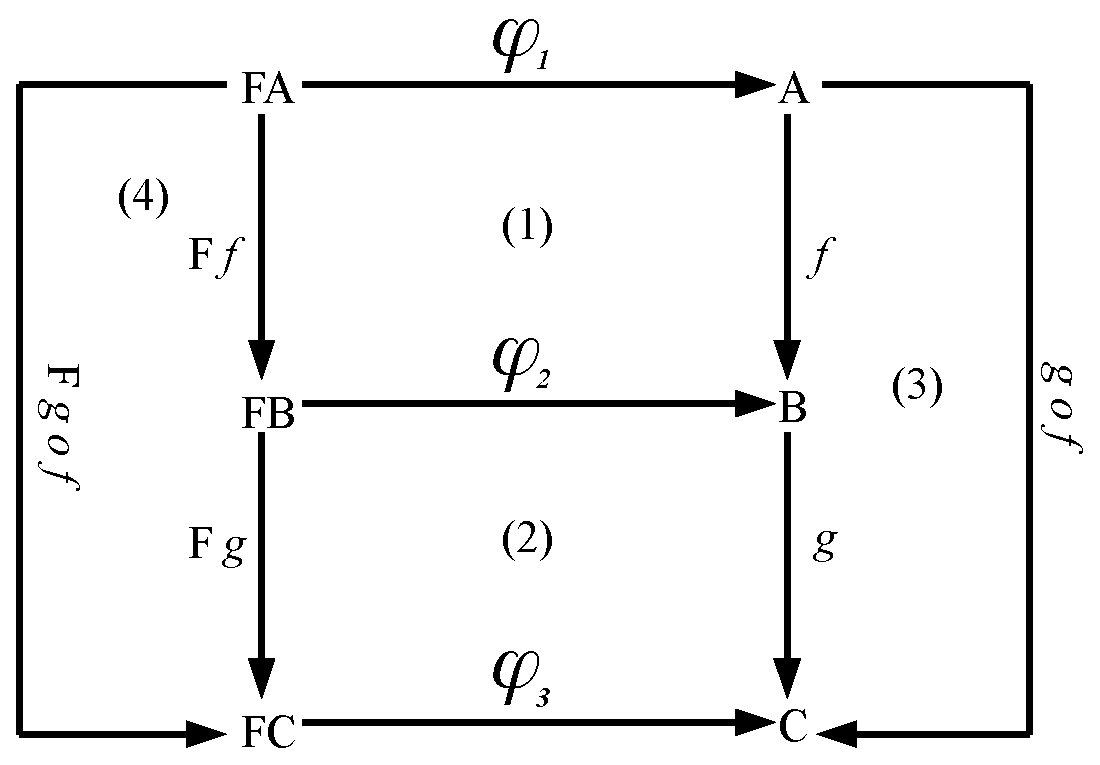
\includegraphics[width=0.5\textwidth]{figures/alg3}
\caption{F-homomorpisms preserved under composition}
\end{center}
\end{figure}


In order to prove that the composition of the F-algebras is a homomorphism, we need to show that the outer diagram commutes.

\begin{proof}
$f$ is an F-homomorphism $\Rightarrow f \circ \varphi_{1} = \varphi_{2} \circ F(f)$  ... (1) \\
$g$ is an F-homomorphism $\Rightarrow g \circ \varphi_{2} = \varphi_{3} \circ F(g)$  ... (2) \\

$(g \circ f) \circ \varphi_{1}$ \\
$= g \circ f \circ \varphi_{1}$ \\
$= g \circ \varphi_{2} \circ F(f)$     (from (1)) \\
$= \varphi_{3} \circ F(g) \circ F(f)$  (from (2)) \\
$= \varphi_{3} \circ F(g \circ f)$   ($F$ is a functor) \\

Hence the outer diagram commutes. Also intuitively:

- diagram (1) commutes    ($f$ is an F-homomorphism) \\
- diagram (2) commutes    ($g$ is an F-homomorphism) \\
- diagram (3) commutes    (by composition) \\
- diagram (4) commutes    (F is a functor)  \\

Hence the outer diagram commutes and $g \circ f$ is also an F-homomorphism.
\end{proof}
}


\end{itemize}

\section{Initial object}

An initial object of a category C is an object I in C such that for every object X in C, there exists precisely one \textit{unique} arrow of type $I \rightarrow X$. Here are examples of initial objects in some categories:

\begin{itemize}
\item{The empty set is the unique initial object in the category of sets since $\{\} \rightarrow A$ is the empty function for any object A in the set}
\item{In the category of semigroups, the empty semigroup is the unique initial object}
\end{itemize}
It's not mandatory that every category has an initial object. For example, a non-empty set does not have an initial object.

\subsection{Uniqueness of initial objects}

If I1 and I2 are both initial objects in the category C, then there's exactly one unique arrow $I1 \rightarrow I2$ and that arrow is an isomorphism. i.e. the initial objects are \textit{uniquely isomorphic}. \\ \\
\begin{proof}
I1 is an initial object in C \\
$\Rightarrow$ for each object X in C, there's a unique arrow $I1 \rightarrow X$ \\
$\Rightarrow$ For $X = I2$ (substituting I2 for X), we have the unique arrow $f: I1 \rightarrow I2$ \\ \\
I2 is also initial \\
$\Rightarrow$ for each object X in C, there's a unique arrow $I2 \rightarrow X$ \\
$\Rightarrow$ For X = I1 (substituting I1 for X), we have the unique arrow $g: I2 \rightarrow I1$ \\ \\
$f \circ g = I2 \rightarrow I2$ (by composition) \\
$g \circ f = I1 \rightarrow I1$ (by composition) \\ \\
$I2 \rightarrow I2 = id_{I2}$ and $I1 \rightarrow I1 = id_{I1}$ (by initiality) \\
$\Rightarrow f \circ g = id_{I2}$ and $g \circ f = id_{I1}$ \\ \\
$\Rightarrow$ There's a bidirectional inverse between f and g since the arrow $I1 \rightarrow I2$ has an inverse arrow $I2 \rightarrow I1$. Hence the unique arrows f and g establish the unique isomorphism. \\ \\
But there's something more. When we say that 2 objects are isomorphic, there may be many isomorphisms establishing that fact between the two objects. But for initial objects, there's only one - hence all initial objects are indistinguishable. So we call \textit{the} initial object rather than \textit{an} initial object of a category. The initial object is usually denoted by 0 and the unique arrow $0 \rightarrow X$ is denoted by !(rev)X (gnab).
\end{proof}

\section{Terminal object}

A terminal object of a category C is an object T in C if for every object X in C there exists a unique arrow $X \rightarrow T$. A category may have more than one terminal objects, but all are isomorphic (like initial objects) and hence we call \textit{the} terminal object. The terminal object is usually denoted by 1 and the unique arrow $X \rightarrow 1$ is denoted by !X (bang). \\ \\
Here are examples of terminal objects in some categories:

\begin{itemize}
\item{Every one-element set (singleton) is a terminal object in this category}
\item{In the category of semigroups, any singleton semigroup is a terminal object}
\end{itemize}
It's not mandatory that every category has a terminal object. For example, The category of simple graphs \footnote{A simple graph is an undirected graph that has no loops and no more than one edge between any two different vertices} does not have a terminal object.

\section{Initial Algebra}

An initial F-algebra is an initial object in the category of F-algebras (Alg(F) defined above). Let's look at it in a bit more detail. In Alg(F) if there exists an F-algebra $\left( \mu F, in\right) $ such that for any F-algebra $\left( C, \varphi\right) $ in that category, there exists a unique arrow $\{\varphi\}: \mu F -> C$ making the following diagram commute.\footnote{Isn't this the precise definition of an initial object?} \\


\begin{figure}[htb]
\begin{center}
\includegraphics[width=0.5\textwidth]{figures/alg4}
\caption{$\{ \varphi \}$ is the catamorphism}
\end{center}
\end{figure}

In the diagram, the unique arrow $\{\varphi\}$ is known as \textit{Catamorphism}. We say that the initial algebra $(\mu F, in)$ is an initial object in the category Alg(F), and the catamorphism $\{\varphi\}$ is the mediating arrow out of it. 

\subsection{Properties of initial F-algebra}

Let $(\mu F, in)$ be an initial F-algebra. Here are some of the laws that apply to initial algebras.

\begin{enumerate}
\item{\textbf{Cancellation:} For any F-algebra $\varphi : FC \rightarrow C$, $\{\varphi\}\, \circ\, in = \varphi\, \circ\, F\, \{\varphi\}$ (follows straight from the diagram)}

\item{\textbf{Reflection:} $id = \{in\}$. Follows from the diagram below, since $\mu F \rightarrow \mu F$ is the id of the algebra.

\begin{figure}[htb]
\begin{center}
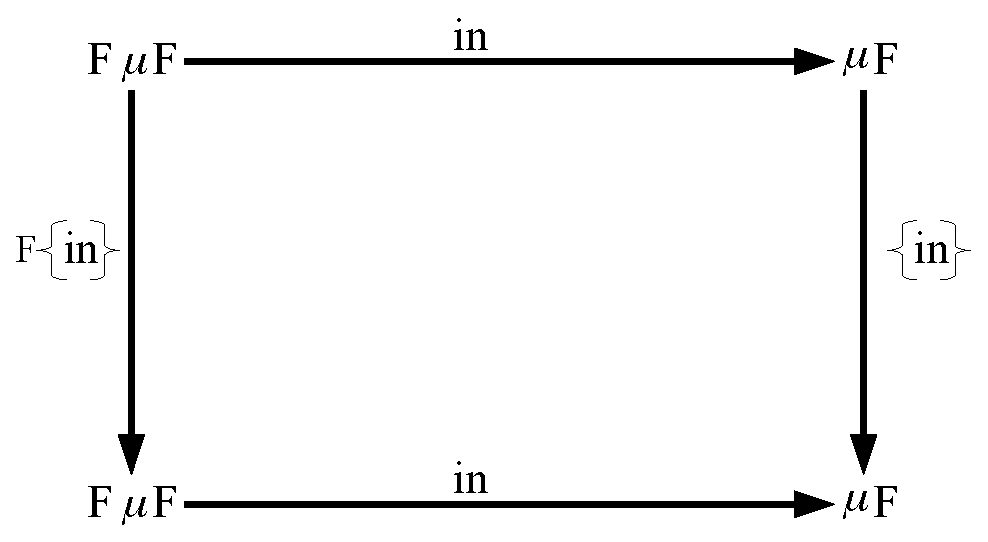
\includegraphics[width=0.5\textwidth]{figures/alg5}
\caption{Reflection in initial F-algebra}
\end{center}
\end{figure}

}
\item{\textbf{Universality:} The diagram for initial F-algebra commutes and we get the following equivalence:
\begin{center}
$f \circ in = \varphi \circ Ff  \Leftrightarrow f = \{\varphi\}$
\end{center}

This is known as the \textit{Universal Property} and finds extensive use in proving various properties of catamorphism. 
}
\item{\textbf{Fusion:} For any two F-algebras $f: FC \rightarrow C$ and $g: FD \rightarrow D$ and an arrow $h: C \rightarrow D$, we have:
\begin{center}
$h \circ f = g \circ F h \Rightarrow h \circ \{f\} = \{g\}$
\end{center}

\begin{proof}
Consider the following diagram:

\begin{figure}[htb]
\begin{center}
\includegraphics[width=0.5\textwidth]{figures/alg6}
\caption{Fusion}
\end{center}
\end{figure}

Here
\begin{itemize}
\item{$(\mu F, in)$ is an initial F-algebra}
\item{$(C, f)$ and $(D, g)$ are F-algebras}
\item{$h: (C, f) \rightarrow (D, g)$ is an F-homomorphism}
\end{itemize}

Then the \textit{fusion} law states that the composition of a homomorphism and catamorphism is again a catamorphism. Here's how we can derive it:

$h \circ \{f\} = \{g\}$ \\ \\
$\Leftrightarrow$ \{universal property\}  \\
$h \circ \{f\} \circ in = \{g\} \circ F( h \circ \{f\} )$ \\ \\
$\Leftrightarrow$ \{F is a functor\} \\
$h \circ \{f\} \circ in = \{g\} \circ Fh \circ F\{f\}$ \\ \\
$\Leftrightarrow$ \{\{f\} is an F-homomorphism\} \\
$h \circ f \circ F\{f\} = \{g\} \circ Fh \circ F\{f\}$ \\ \\
$\Leftrightarrow$ \{cancellation\} \\
$h \circ f        = \{g\} \circ Fh$ \\ \\
$\Leftrightarrow$ \{h is an F-homomorphism\} \\
true
\end{proof}
}


\item{\textbf{Isomorphism:} The initial algebra $(\mu F, in)$ for an endofunctor F in category C defined as $in : F \mu F \rightarrow \mu F$ is an isomorphism. i.e $\mu F$ is isomorphic to $F \mu F$ via $in$, with the inverse defined as $in ^{-1} : \{F\, in\}$. This is the Lambek's theorem.

\begin{proof}
We need to show that in is the pre and post inverse of $in ^{-1}$.

$\Longrightarrow$ pre \\
$in \circ in ^{-1}$  \\
$=  in \circ \{F\, in\}$  \\ \\
$=$  \{fusion law\}  \\
$   \{in\}$  \\ \\
$=$  \{reflection\}  \\
$   id$ \\

$\Longrightarrow$ post \\
$in ^{-1} \circ in$ \\
$=  \{F\, in\} \circ in$ \\ \\
$=$  \{cancellation\} \\
$   F\, in \circ F \{F\, in\}$ \\ \\
$=$  \{F is a functor\} \\
$   F (in \circ \{F\, in\})$ \\ \\
$=$  {from pre} \\
$   F\, id$ \\ \\
$=$  {F is a functor} \\
$   id$ \\
\end{proof}
In the above initial algebra we have $\mu F$ as the carrier and it defines an isomorphism. This means the carrier of the initial algebra is (up to isomorphism) a fixed point of the functor.
}

\end{enumerate}

\section{Initial Algebra and Recursive Data Types}

An initial algebra generalizes the notion of a recursive data type. Consider a List data type which can be represented by the following Sum type: \\ \\
// nil takes no arguments and returns a List data type \\
$nil: 1 \rightarrow List[A]$ \\ \\
// cons takes 2 arguments and returns a List data type \\
$cons: (A \times List[A]) \rightarrow List[A]$ \\ \\
Combining the 2 functions we get: \\ \\
$in = [nil, cons]: 1 + (A \times List[A]) \rightarrow List[A]$, which translates to the functor $LA(X) = 1 + (A \times X)$. So the data type of lists over the set A can be represented as an initial F-algebra $(\mu LA, in)$ over the functor LA. Here we write $\mu LA$ for List[A]. Let's prove it. \\ \\
In order that $(\mu LA, in)$ is an initial algebra, we need to show that for an arbitrary F-algebra $(C, \varphi)$, where $\varphi$ is an arrow out of the sum type given by : \\ \\
$c: 1 \rightarrow C$ \\
$h: (A \times C) \rightarrow C$ \\ \\
and the join gives :
$[c, h]: 1 + (A \times C) \rightarrow C$ \\ \\
Here's the category diagram
\begin{figure}[htb]
\begin{center}
\includegraphics[width=0.5\textwidth]{figures/alg7}
\caption{List as initial F-algebra}
\end{center}
\end{figure}
In order for $(\mu LA, in)$ to be an initial F-algebra, we need to find a homomorphism $f: \mu LA \rightarrow C$ and show that it is unique. Doing this we will be able to find the initial object for the initial algebra. f will be a homomorphism if the above diagram commutes, for which we need : \\ \\
$f \circ nil = c$  and \\
$f \circ cons = h \circ (id x f)$ \\ \\
From the Universal property of initial F-algebras discussed above, it's easy to see that this system of equations has a unique solution which is fold(c, h) [try it as an exercise]. It's the catamorphism represented by: \\ \\
\begin{center}
 $f: \{ [c, h] \} : List[A] \rightarrow C$
\end{center}
This proves our initial hypothesis that $\mu LA$ is an initial F-algebra over the endofunctor $F: LA(X) = 1 + (A \times X)$. \\ \\
Treating List as an initial F-algebra lets us define many of the list properties algebraically in terms of catamorphism. Consider length of a List, which is defined as $length: List[A] \rightarrow Nat$, where Nat is the set of natural numbers defined with its zero and successor functions as follows: \\ \\
$zero: 1 \rightarrow Nat$ \\
$succ: Nat \rightarrow Nat$ \\ \\
We can define \textit{length} as a catamorphism : $length = \{ [zero, \lambda(a, n).succ(n)] \}$. \\ \\
Similarly for $concat: List[A] \times List[A] \rightarrow List[A]$, we can define it in terms of catamorphism as:

\begin{center}
$concat(xs, ys) = \{ [\lambda(x).ys, cons] \}(xs)$
\end{center}

When we talk about algebraic data types, we need to understand the algebra that goes with it. We can consider any algebraic data type as an initial F-algebra on the endofunctor F.



\end{document}